% This version of CVPR template is provided by Ming-Ming Cheng.
% Please leave an issue if you found a bug:
% https://github.com/MCG-NKU/CVPR_Template.

%\documentclass[review]{cvpr}
\documentclass[final]{cvpr}

\usepackage{times}
\usepackage{epsfig}
\usepackage{graphicx}
\usepackage{amsmath}
\usepackage{amssymb}

% Include other packages here, before hyperref.

% If you comment hyperref and then uncomment it, you should delete
% egpaper.aux before re-running latex.  (Or just hit 'q' on the first latex
% run, let it finish, and you should be clear).
\usepackage[pagebackref=true,breaklinks=true,colorlinks,bookmarks=false]{hyperref}

\usepackage{subcaption}
\usepackage{fontspec}
\setmainfont{TeX Gyre Termes}


\def\cvprPaperID{****} % *** Enter the CVPR Paper ID here
\def\confYear{CVPR 2021}
%\setcounter{page}{4321} % For final version only


\begin{document}

%%%%%%%%% TITLE
\title{Lecture Node for Seam Carving}

\author{Zhengyang Gu
Sun Yat-sen University
{\tt\small guzhy3@mail2.sysu.edu.cn}
% For a paper whose authors are all at the same institution,
% omit the following lines up until the closing ``}''.
% Additional authors and addresses can be added with ``\and'',
% just like the second author.
% To save space, use either the email address or home page, not both
}
\maketitle


%%%%%%%%% ABSTRACT
\begin{abstract}
    The lecture gave us some basic concepts about seam carving, which are very intriguing.
    Therefore, I read the papper\cite{avidan2007seam} which first introduce seam carving and some other related pappers, in order to dig deeper into this algorithm.
\end{abstract}

%%%%%%%%% BODY TEXT
\section{Introduction}
Image retargeting is to change the size of pictures on a website when the website is accessed by different divices with various screen sizes.
The simplest way is scaling and cropping\ref{fig:gibbous_scale_crop}.
However, scaling may distort important contents in pictures.
For example, the cat\ref{fig:gibbous_scale_crop} becomes obviously distorted after scaling.
And cropping may remove important contents at the periphery of pictures.
For instance, some of the tentacles near the edges of the picture\ref{fig:gibbous_scale_crop} are removed.
Therefore, content-aware image resizing approaches that can maintain important contents when resizing pictures is in great demand.
\begin{figure}[htb]
\begin{center}
\begin{subfigure}[b]{0.768\linewidth}
    
\includegraphics[width=\textwidth]{gibbous.jpg}
    \caption{Original}
\end{subfigure}
\begin{subfigure}[b]{0.48\linewidth}
    
\includegraphics[width=\textwidth]{gibbous_scaling.jpg}
    \caption{Scaling}
\end{subfigure}
\begin{subfigure}[b]{0.48\linewidth}
    
\includegraphics[width=\textwidth]{gibbous_cropping.jpg}
    \caption{Cropping}
\end{subfigure}
\end{center}
\caption{The original picture shows a cat with some tentacles. The picture is scaled and cropped.}
\label{fig:gibbous_scale_crop}
\end{figure}

Seam carving is a content-aware image resizing apporach.
The basic idea of it is to remove the most unimportant pixels in a seam which is intuitively a line.
Therefore, it can eliminate redundance and keep consistency of pictures at the same time.
For example, the picture\ref{fig:gibbous_seam_carve} is resized by seam carving, while the cat is not distorted and the tentacles are not removed.
\begin{figure}[htb]
\begin{center}
    
\includegraphics[width=0.48\linewidth]{gibbous_seam_carving.jpg}
\end{center}
\caption{Seam carving}
\label{fig:gibbous_seam_carve}
\end{figure}
\section{Background}
There are some other content-aware image resizing methods mentioned by the paper\cite{avidan2007seam}.
For example, use top down methods like face detectors\cite{viola2001rapid} or bottom down methods like visual saliency methods\cite{itti1998model} to build saliency map.
And then based on the saliency map, use intelligent cropping methods to resize the image\cite{suh2003automatic}.
Another paper\cite{chen2003visual} pays attention to users' perception on the adapted images.
Their method automatically detect and transmit the most important part of the image to devices.

And the paper\cite{avidan2007seam} also mentioned other areas where seams are used.
For instance, the paper\cite{agarwala2004interactive} finds the best seams to combine parts of a set of pictures into a single composite picture.
And the computation of seams can be done by other ways, including Dijkstra's shortest path algorithm\cite{davis1998mosaics} and graph cuts\cite{boykov2001interactive}.
\section{Theory}
\subsection{Energy Functions}
Since we want to delete those pixels that are unimportant, we need to have a method to evaluate the importance of pixels.
This leads to the definition of energy function, which has the form of
\begin{equation}
    e(\textbf I),\text{s.t.}\forall i,j\in\mathbb{N}\wedge i<m\wedge j<n,e(\textbf I(i,j))\ge0,
    \label{eq:energy_function}
\end{equation}
where $\textbf I$ is an image with the size of $m\times n$.
If a pixel is of less importance than another pixel, it has lower energy than the other pixel.
The papper\cite{avidan2007seam} gives several energy functions and compares their performance.
It finds that no single energy function  well on all pictures and either the $e_1$ or $e_{HoG}$ performs well.
\subsubsection{The $e_1$}
$e_1$\ref{eq:e1} is the simplest energy function.
It's the $L_1$-norm of the gradient, which has the form of
\begin{equation}
    e_1(\textbf{I})=\left|\frac\partial{\partial x}\textbf I\right|+\left|\frac\partial{\partial y}\textbf I\right|.
    \label{eq:e1}
\end{equation}
And it's actually an edge-detector, which means that if a pixel is on an edge, it has large $e_1$, while if the pixel is on a plain, it has low $e_1$.
The basic idea of it is that pixels on edges contain more information of the picture than pixels on plains.
Therefore, pixels on edges are of more importance, so we try to preserve pixels on edges and remove pixels on plains in order to preserve as much information as possible.

$e_1$\ref{eq:e1} ensures that pixels removed don't appear on edges.
However, chances are that many pixels inside objects are removed, which may distort objects in images.
In addition, winding edges may become straight because of that.
Approaches to solve this problem are as follows.
\subsubsection{Energy Functions With Masks}
There is a simpler way to solve the problem.
Let's go back to the definition of energy function\ref{eq:energy_function}.
What we want to do is try not to remove pixels inside the objects, and what we always do is to remove pixels with low energy.
Therefore, we can mannually make masks on objects or use some other approaches like the output of face detector to make masks, and increase energy of pixels in masks.
As a result, those pixels that are masked are protected from being removed.

This set of pictures\ref{fig:gibbous_seam_carving_mask} illustrates how mask works to prevent important objects from being distorted.
The white space is the space to be protected.
The cat and its tentacles are protected by masks from being distorted compared with output of the seam carving.
\begin{figure}[htb]
\begin{center}
\begin{subfigure}[b]{0.768\linewidth}
    
\includegraphics[width=\textwidth]{gibbous.jpg}
    \caption{Original}
\end{subfigure}
\begin{subfigure}[b]{0.768\linewidth}
    
\includegraphics[width=\textwidth]{gibbous_mask.jpg}
    \caption{Mask}
\end{subfigure}
\begin{subfigure}[b]{0.48\linewidth}
    
\includegraphics[width=\textwidth]{gibbous_seam_carving_without_mask.jpg}
    \caption{Seam carving without masks}
\end{subfigure}
\begin{subfigure}[b]{0.48\linewidth}
    
\includegraphics[width=\textwidth]{gibbous_seam_carving.jpg}
    \caption{Seam carving with masks}
\end{subfigure}
\end{center}
\caption{Comparison between seam carving without masks and with masks}
\label{fig:gibbous_seam_carving_mask}
\end{figure}
\subsubsection{The $e_{HoG}$}
$e_{HoG}$\ref{eq:eHoG} adopts histogram of oriented gradients\cite{dalal2005histograms} to penalize pixels that are near edges.
Intuitively, $HoG(\textbf I(x,y))$ is a vector recording counts of pixel $I(x,y)$'s neighbors' gradients' orientations.
If a pixel is near an edge, most of its neighbors will have the same gradients' orientations, so $\max(HoG(\textbf I(x,y)))$ will be high.
On the other hand, if the pixel is far from edges which means it locates inside of a object, its neighbors' gradients will orient randomly, so $\max(HoG(\textbf I(x,y)))$ will be low.

Based on this fact, the paper\cite{avidan2007seam} defines $e_{HoG}$\ref{eq:eHoG} as
\begin{equation}
    e_{HoG}(\textbf{I(x,y)})=\frac{e_1(\textbf{I(x,y)})}{\max(HoG(\textbf I))}.
    \label{eq:eHoG}
\end{equation}
It\ref{eq:eHoG} ensures that pixels removed tend to edges.
In this way, the curves on edges can be preserved.

For instance, the moon in the set of pictures\ref{fig:cloud_seam_carving_HoG} that is processed by $E_{HoG}$ better preserved its curves.
\begin{figure}[htb]
\begin{center}
\begin{subfigure}[b]{0.768\linewidth}
    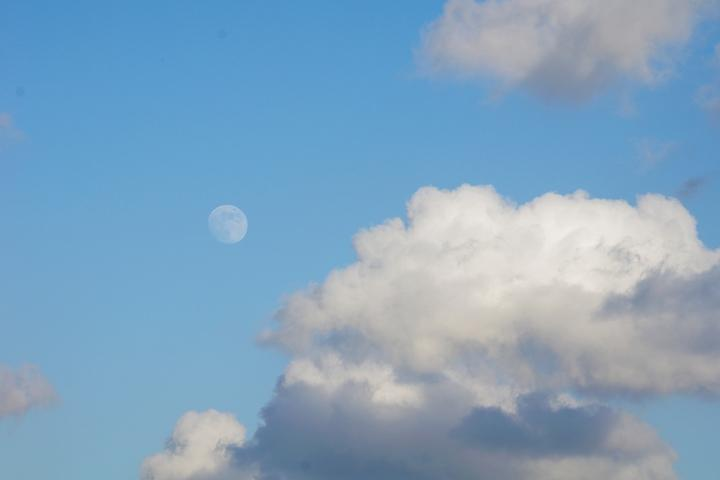
\includegraphics[width=\textwidth]{cloud.jpg}
    \caption{Original}
\end{subfigure}
\begin{subfigure}[b]{0.48\linewidth}
    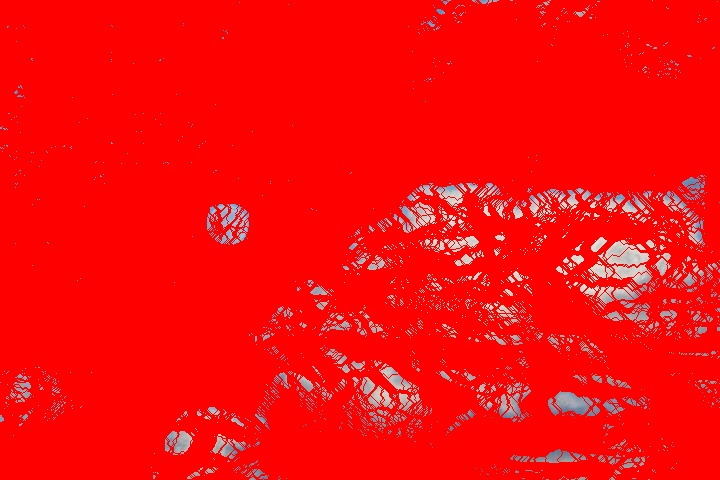
\includegraphics[width=\textwidth]{cloud_seam_carving_records.jpg}
    
\includegraphics[width=\textwidth]{cloud_seam_carving.jpg}
    \caption{The result of seam carving using $e_1$}
\end{subfigure}
\begin{subfigure}[b]{0.48\linewidth}
    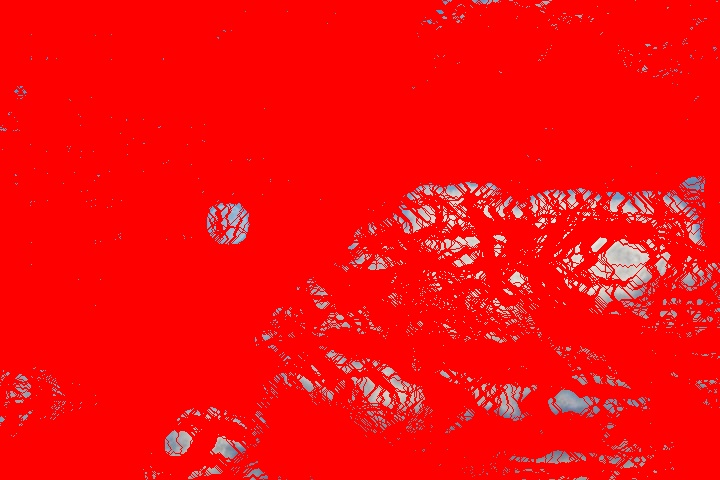
\includegraphics[width=\textwidth]{cloud_seam_carving_HoG_records.jpg}
    
\includegraphics[width=\textwidth]{cloud_seam_carving_HoG.jpg}
    \caption{The result of seam carving using $e_{HoG}$}
\end{subfigure}
\end{center}
\caption{Comparison between energy function $e_1$ and $e_{HoG}$}
\label{fig:cloud_seam_carving_HoG}
\end{figure}
\subsection{Seams}
Generally, we want to remove pixels with low energy.
However, just choosing those pixels that have the lowest energy to remove can be a very bad strategy.
That is because pixels with the lowest energy can be randomly scattered across the whole picture, which means deleting them may destroy the rectangle shape of the picture.
There are several other strategies to choose pixels to remove.

Removing pixels in seams is the best approach according to the papper\cite{avidan2007seam}.
Seams are intuitively constant lines linked\ref{eq:adjacency} by pixels.
Therefore, they can help to preserve the consistency and the rectangle shape of the picture very well.
Adjacency is defined as
\begin{equation}
    \begin{cases}
        0\le|x_1-x_2|\le1\wedge0<|y_1-y_2|\le1\\
        0<|x_1-x_2|\le1\wedge0\le|y_1-y_2|\le1
    \end{cases},
    \label{eq:adjacency}
\end{equation}
which can be be shown in pictures\ref{fig:adjacency}.
\begin{figure}[htb]
\begin{center}
\begin{subfigure}[b]{0.30\linewidth}
    
\includegraphics[width=\textwidth]{to_right.png}
\end{subfigure}
\begin{subfigure}[b]{0.30\linewidth}
    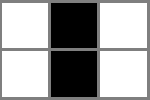
\includegraphics[width=\textwidth]{straight.png}
\end{subfigure}
\begin{subfigure}[b]{0.30\linewidth}
    
\includegraphics[width=\textwidth]{to_left.png}
\end{subfigure}
\end{center}
\caption{Three cases of adjacency}
\label{fig:adjacency}
\end{figure}

Assume that $\textbf{I}$ is an $n\times m$ image.
Vertical seams are defined as
\begin{equation}
    \textbf s^\textbf x=\{s^x_i\}_{i=1}^n,\text{s.t.}\forall i,|x(i)-x(i-1)|\le1,
    \label{eq:vertical_seam}
\end{equation}
and horizontal seams are defined as
\begin{equation}
    \textbf s^\textbf y=\{s^y_j\}_{j=1}^m,\text{s.t.}\forall j,|y(j)-y(j-1)|\le1.
    \label{eq:horizontal_seam}
\end{equation}
The pixels on the seam $\textbf s$ are hence
\begin{equation}
    \textbf I_\textbf s=\{I(s^x_i)\}_{i=1}^n=\{I(x(i),i)\}.
    \label{eq:pixel_on_vertical_seam}
\end{equation}

Given an energy function $e$, the cost of the seam can be defined as
\begin{equation}
    E(\textbf s)=E(\textbf I_\textbf s)=\sum_{i=1}^ne(\textbf I(s_i)).
    \label{eq:energy_of_seam}
\end{equation}
Therefore, the problem can be converted into finding the path with the lowest cost on a graph, which is to find
\begin{equation}
    \textbf s^*=\arg\min\limits_\textbf sE(\textbf s).
    \label{eq:solution_of_optimal_seam}
\end{equation}
\section{Implementations}
\subsection{Dynamic Programming}
Dynamic programming can be adopted to find seams.
We define $M(i,j)$ to be the cumulative minimum energy among all possible paths reaching the point$(i,j)$.
The state transition function can be written as
\begin{equation}
    \begin{aligned}
        M(i,j)=e(i,j)+\min(M(i-1,j-1),M(i-1,j),\\
        M(i-1,j+1)),
    \end{aligned}
    \label{eq:M0}
\end{equation}
where the image has the size of $m\times n$ and $1\le i\le m-1\wedge 1\le j\le n-2$.
When $1\le i\le m-1\wedge j=0$, the state transition function has the form of
\begin{equation}
    M(i,j)=e(i,j)+\min(M(i-1,j),M(i-1,j+1)).
    \label{eq:M1}
\end{equation}
When $1\le i\le m-1\wedge j=n-1$, the state transition function has the form of
\begin{equation}
    M(i,j)=e(i,j)+\min(M(i-1,j-1),M(i-1,j)).
    \label{eq:M2}
\end{equation}
And the initial state has the form of
\begin{equation}
    M(i,j)=e(i,j),
    \label{eq:M3}
\end{equation}
where $i=0\wedge 0\le j\le n-1$.

After calculating $M(i,j),\text{s.t.}\forall 0\le i\le m-1\wedge0\le j\le n-1$, we can find the optimal seam by calculating
\begin{equation}
    \min M(m-1,j),\text{s.t.}\forall0\le j\le n-1.
    \label{eq:minM}
\end{equation}

Time complexity for calculating $M(i,j),\forall 0\le i\le m-1\wedge0\le j\le n-1$ is $O(mn)$.
And time complexity for calculating $\min M(m-1,j),\text{s.t.}\forall0\le j\le n-1$ is $O(n)$.
Therefore, time coplexity for finding the optimal seam is $O(mn)$.

Additionally, there is a detail that can help to improve the spacial efficiency of the dynamic programming.
The matrix with the size of $m\times n$ that is used to store $M(i,j)$ can be reduced to an array $A$ with the size of $1\times n$.
Initially, $A$ stores the initial state\ref{eq:M3}.
When calculating other $M(i,j)$, we store $M(i,j)$ into $A(j)$ only after having calculated $M(i,j+2)$.
That is because after the calculation of $M(i,j+2)$, the $M(i-1,j)$ that is stored in $A(j)$ will no longer be accessed.
\subsection{Reuse Of Energy Map}
The energy map that have already been computed can be reused under some circumstances.
Suppose that the energy function $e_1(\textbf I)$\ref{eq:e1} is calculated by sobel operator.
The calculation of $e_1(i,j)$ can be written as
\begin{equation}
    \begin{aligned}
        e_1(\textbf{I})=&\left|\frac\partial{\partial x}\textbf I\right|+\left|\frac\partial{\partial y}\textbf I\right|\\
        =&\left|
        \begin{bmatrix}
            -1 & 0 & 1\\
            -2 & 0 & 2\\
            -1 & 0 & 1
        \end{bmatrix}
        *\textbf I(i-1:i+1,j-1:j+1)\right|\\
        +&\left|
        \begin{bmatrix}
            -1 & -2 & -1\\
            0 & 0 & 0\\
            1 & 2 & 1
        \end{bmatrix}
        *\textbf I(i-1:i+1,j-1:j+1)\right|\\
    \end{aligned}.
    \label{eq:sobel}
\end{equation}
Therefore, the only dependence when calculating $e(\textbf I(i,j))$ is $\textbf I(i+x,j+y),\forall -1\le x,y\le 1$.
Hence, after removing a pixel$(i,j)$, only the energy of those pixels in $(i,j)$'s neighborhood
\begin{equation}
    \{(x,y)|\forall x\in[i-1,i+1]\wedge y\in[j-1,j+1]\}
    \label{eq:neighborhood}
\end{equation}
will be affected. And reuse the rest of energy map can greatly enhance the efficiency.
\subsection{Real Time Computation}
Seam carving can be used to solve the image retargeting problem in web designing.
It is not uncommon that sizes of target images are unkown, resulting from that web users may use devices with various size of monitors, which may use different resolutions when accessing the website.
Therefore, the efficiency of resizing a single image embedded in a web page into several sizes is very important.

Real time computation can be realized because of the constraint that only a single image.
We can resize the image into several sizes that are potentially in need and store the process of resizing.
Supposing that we want to resize a image with the size of $m\times n$ into $m'\times n$ where $m_{\min}\le m'<m$.
We can build a matrix with the size of $m\times n$ which will be used to store the orders of seams to be removed.
Then we resize the image into the height $m_{\min}$.
Everytime we remove a pixel, we fill in the matrix with the index of which of the seams the pixel belongs to.
After building the matrix, if we want to resize the image into the size of $m'\times n$, we can remove seams as the order recorded in the matrix without the calculattion of energy map or the optimal path.
We can see from the experiment\ref{fig:dolphin_seam_carve}\ref{fig:dolphin_seam_carve_output} that seam carving with records is greatly faster than that without records.
\begin{figure}[htb]
\begin{center}
    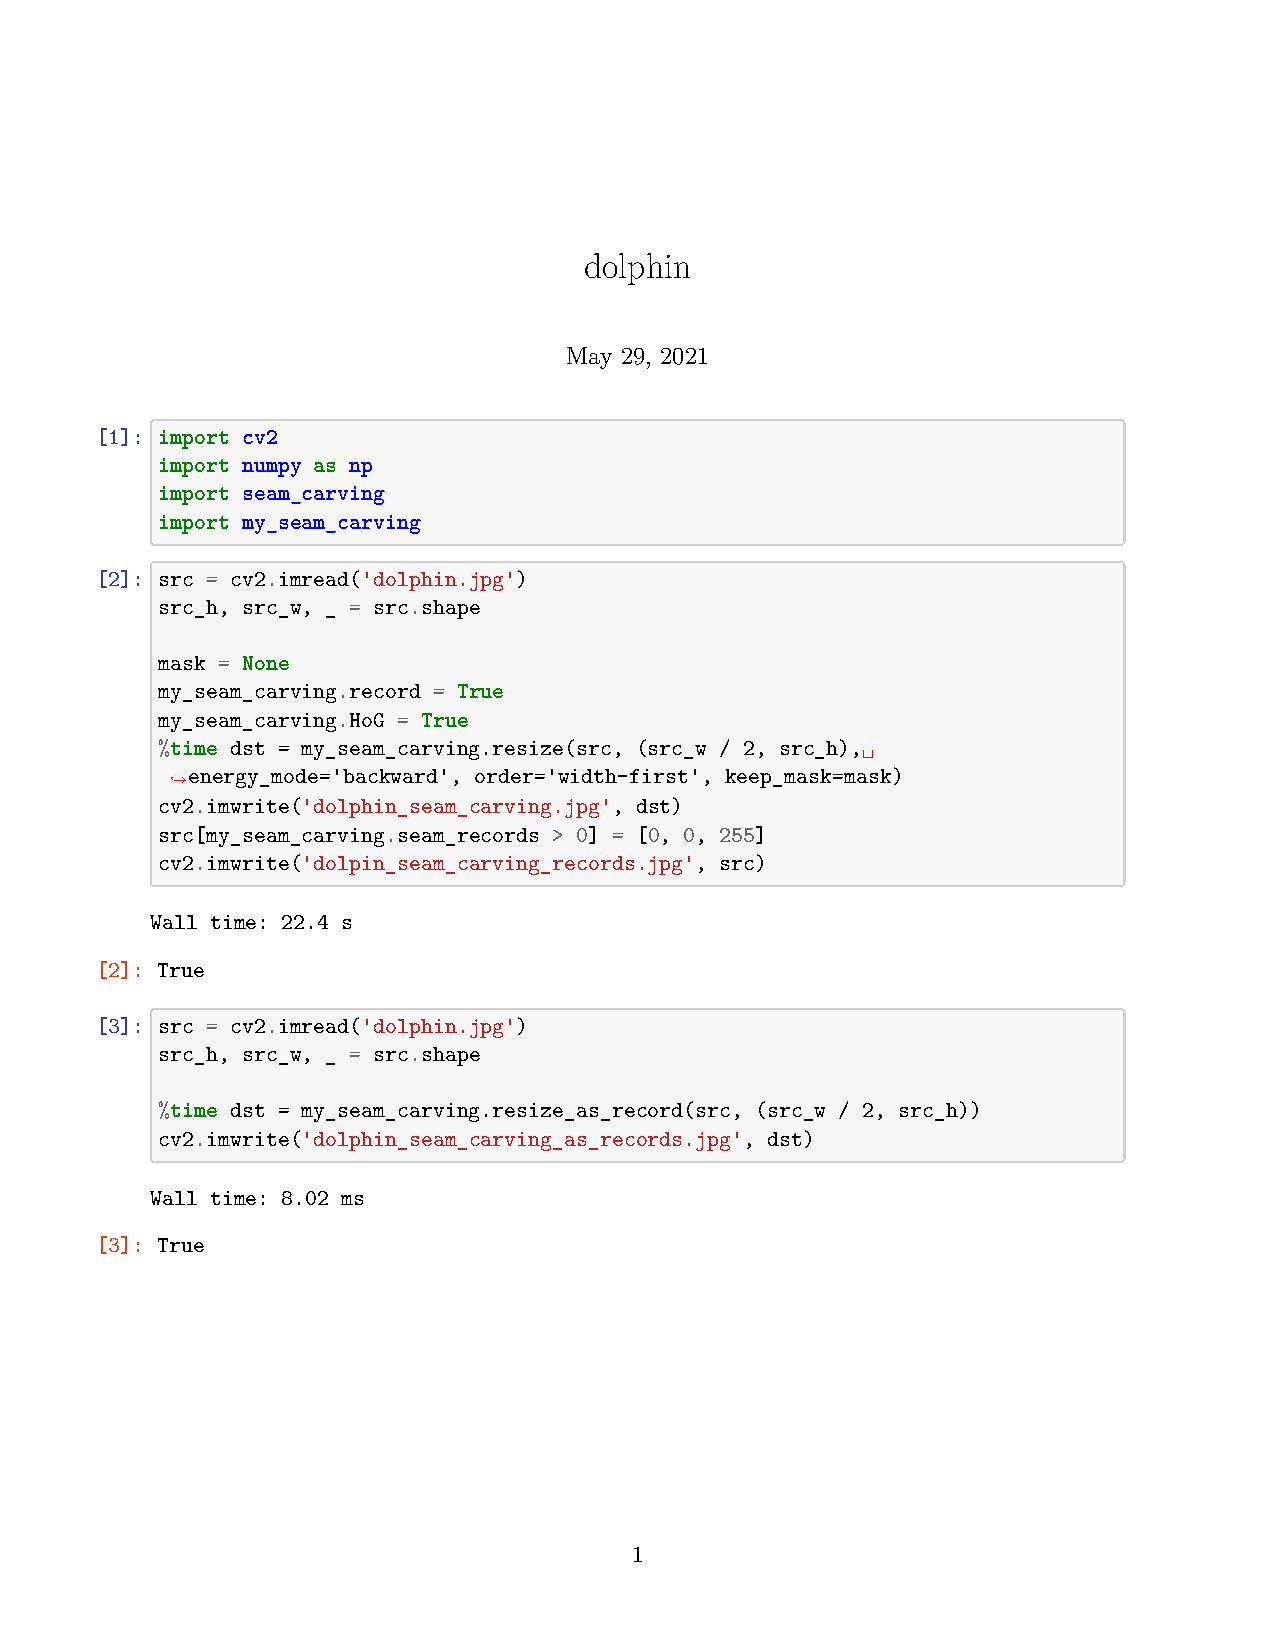
\includegraphics[width=\linewidth]{dolphin.pdf}
\end{center}
\caption{Efficiency comparison between resizing without and with records}
\label{fig:dolphin_seam_carve}
\end{figure}
\begin{figure}[htb]
\begin{center}
\begin{subfigure}[t]{0.48\linewidth}
    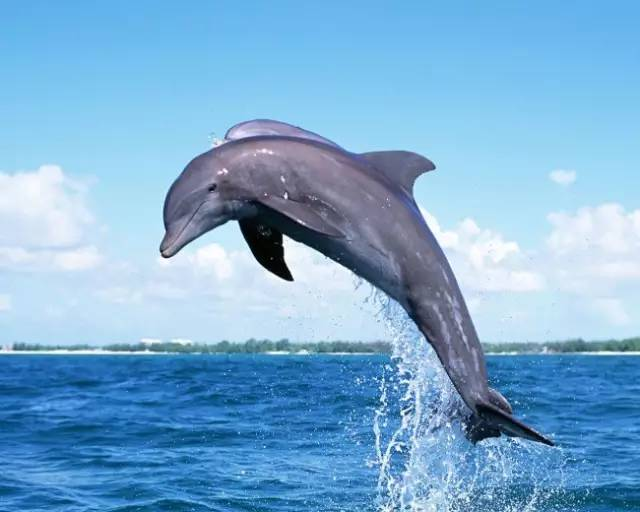
\includegraphics[width=\textwidth]{dolphin.jpg}
    \caption{Original picture}
\end{subfigure}
\begin{subfigure}[t]{0.48\linewidth}
    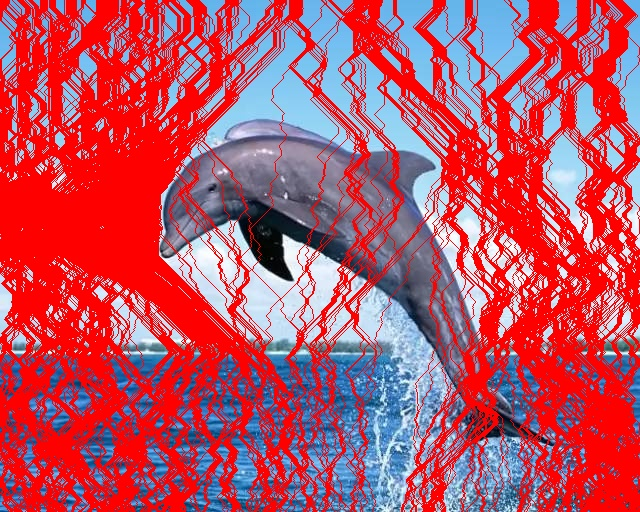
\includegraphics[width=\textwidth]{dolpin_seam_carving_records.jpg}
    \caption{Seam records are marked on the original picture}
\end{subfigure}
\begin{subfigure}[b]{0.24\linewidth}
    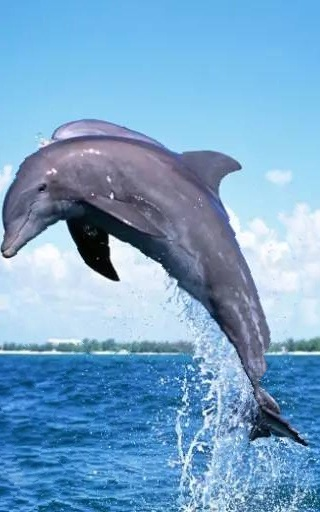
\includegraphics[width=\textwidth]{dolphin_seam_carving.jpg}
    \caption{Seam carving without records}
\end{subfigure}
\begin{subfigure}[b]{0.24\linewidth}
    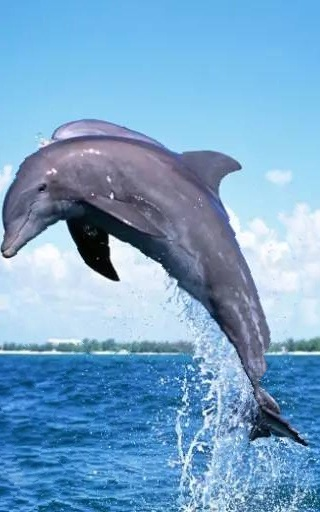
\includegraphics[width=\textwidth]{dolphin_seam_carving_as_records.jpg}
    \caption{Seam carving with records}
\end{subfigure}
\end{center}
\caption{The output of the experiment\ref{fig:dolphin_seam_carve}}
\label{fig:dolphin_seam_carve_output}
\end{figure}

However, if we want to resize the image in 2 dimensions the method won't work.
That is because, vertical seams\ref{eq:vertical_seam} and horizontal seams\ref{eq:horizontal_seam} may colide in many pixels.
Removing a vertical seam may destroy the index map in the horizontal direction and vice versa.
The papper\cite{avidan2007seam} gives a method to solve this problem.
The method is to use degenerate seams, i.e. rows or columns in the other direction.
\subsection{Parallelization}
\subsubsection{Parallelization of previous algorithm}
The process to find the path with the lowest energy can be parallelized.

According to the state transition function\ref{eq:M0}\ref{eq:M1}\ref{eq:M2}, when we are computing $M(i,j)$, the only dependence is $M(i-1,j+x),x=-1,0,1$.
Therefore, it is obvious that the computation within one row $M(i,x),\forall 0\le x\le n-1$ can be parallelized.
However, parallelization among rows is hard to implement, since the computation of each row relies on last row's results.
This parallelization decreases the time coplexity for computing $M(i,j)$ to $O(m)$.

And the calculationg of $\min M(m-1,j),\text{s.t.}\forall0\le j\le n-1$ can be also parallelized.
The calculation is actually finding the minimum of a set.
Assuming that we want to find the minimum of set $S$, the calculation can be done recursively through
\begin{equation}
    \min(S)=\min(\min(S_1),\min(S_2)),\text{s.t.}S=S_1\cup S_2,
    \label{eq:S_minimum}
\end{equation}
where $\min(S_1)$ and $\min(S_2)$ can be computed asynchronously.
And if we want to minimize and balance each workers' work, we'd better have $S_1,S_2$ satisfying
\begin{equation}
    \begin{cases}
        |S_1|=|S_2|\\
        S_1\cap S_2=\emptyset
    \end{cases}.
    \label{eq:division_constraint}
\end{equation}
In this case\ref{eq:division_constraint}, the time complexity for the computation of $\min(S)$ is $\log_2(|S|)$.
Therefore, the time complexity for calculating $\min M(m-1,j),\text{s.t.}\forall0\le j\le n-1$ can be reduced to $O(\log_2(n))$
The time complexity for the whole process of finding the optimal seam can be reduced to
\begin{equation}
    O(m+\log_2(n)).
    \label{eq:M_time_complexity}
\end{equation}
\subsubsection{Another algorithm better suiting parallelization}
The parallelization above seems be a great impovement, but there is another way of dynamic programming for finding the optimal seams that can better take advantage of parallelization.
The state $M(i,j)$ defined above is the minimal cost of seams that reach the point $(i,j)$.
Here we define states $N(i_0,j_0,i_1,j_1),\text{s.t.}\forall0\le i_0,i_1\le m-1\wedge0\le j_0,j_1\le n-1$ as the minimal cost of seams that start from the point $(i_0,j_0)$ and end with the point $(i_1,j_1)$.
The state transition function can be written as
\begin{equation}
    \begin{aligned}
    N(i_0,j_0,i_2,j_2)=&\min\limits_{j_1,x}(N(i_0,j_0,i_1,j_1)+N(i_1,j_1+x,i_2,j_2)),\\
    &\text{s.t.}\forall x\in [-1,1]\\
    &\wedge(i_1,j_1)\in[i_0+1,i_1-1]\times[0,n-1]\\
    &\wedge(i_1,j_1+x)\in[i_0+1,i_1-1]\times[0,n-1].
    \end{aligned}
    \label{eq:N_transition_function}
\end{equation}
And the inial state is
\begin{equation}
    M(i_0,j_0,i_0,j_0)=e(i_0,j_0)
    \label{eq:N_initial_state}
\end{equation}
The advantage of this method is that we can asynchronously compute $N(i_0,j_0,i_1,j_1),\text{s.t.}i_1-i_0=C$ where $C$ is a constant.
Firstly, we compute initial state\ref{eq:N_initial_state}, which is actually $N(i_0,j_0,i_1,j_1),\text{s.t.}i_1-i_0=0$.
Then iteratively, every worker calculates $N(i_0,j_0,i_1,j_1),\text{s.t.}i_1-i_0=C+1$ using state transition function\ref{eq:N_transition_function}.
After the calculation of $N(i_0,j_0,i_1,j_1),\text{s.t.}i_1-j_1=m-1$, the optimal seam can be found through calculating $\min\limits_{j_0,j_1}(N(0,j_0,m-1,j_1))$.

Now let's analyze the time complexity for this algorithm.
Before the analysis, we must know that this algorithm can be viewed in another perspective.
It's actually an application of divide-and-conquer algorithm.
We divide the image vertically into several subimages, separately calculate optimal seams for all the subimages, and then merge subimages and their optimal seams into bigger images and longer seams.
Assume that we want to merge 2 adjacent images with the size of $m_k\times n$ into an image with the size of $2m_k\times n$\ref{fig:merge}.
Every worker works on a unique $(i_0,j_0),(i_1,j_1)$ pair to find minimal seam starting from $(i_0,j_0)$ and ending with $(i_1,j_1)$, which is actually to connect seams in one subimage that start from $(i_0,j_0)$ with adjacent seams in the other subimage that end with $(i_1,j_1)$ and to find the best seam after connection.
And as shown in the schematic diagram\ref{fig:merge}, the number of both seams that start from $(i_0,j_0)$ and seam that end with $(i_1,j_1)$ are at most $2m_k$.
And each seam can be connected with 3 seams to generate 3 longer seams because of 3 types of adjacency\ref{fig:adjacency}.
Therefore, the number of seams starting from $(i_0,j_0)$ and ending with $(i_1,j_1)$ after connection is at most $6m_k$.
Hence, each worker has to find the seam with lowest energy among at most $6m_k$ seams.
And this process of finding the minimal number witin $6m_k$ numbers\ref{eq:S_minimum} can be done parallelly in $O(\log_2(6m_k))$ time complexity, according to the discussion above.
\begin{figure}[htb]
\begin{center}
    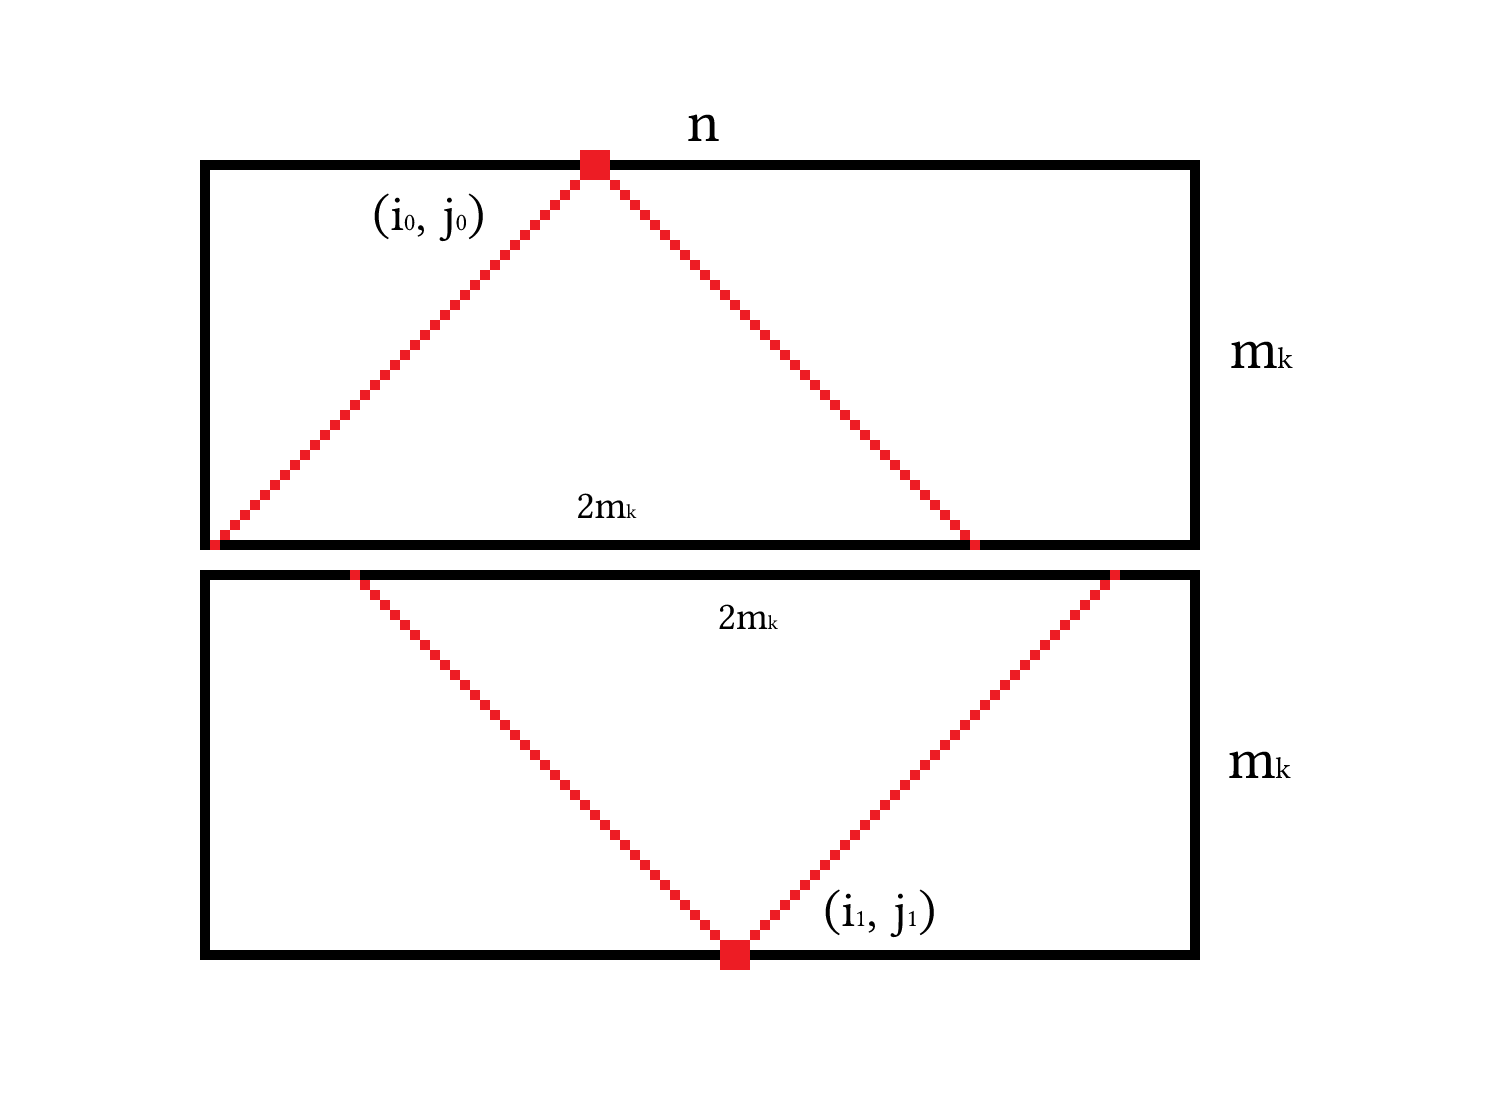
\includegraphics[width=\linewidth]{merge.png}
\end{center}
\caption{Merge 2 adjacent subimages into a bigger image}
\label{fig:merge}
\end{figure}
The original image can be splitted $\log_2(m)$ times.
Therefore the time complexity for calculating $N(0,j_0,m-1,j_1),{s.t.}\forall j_0,j_1\in [0,n-1]$ is
\begin{equation}
    \begin{aligned}
        &O(\sum_{k=1}^{\log_2(m)}(\log_2(6m_k)))\\
        =&O(\sum_{k=1}^{\log_2(m)}(\log_2(6\cdot 2^{k-1})))\\
        =&O(\sum_{k=1}^{\log_2(m)}(k-1+\log_2(6)))\\
        =&O((\log_2(m))^2)
        \label{eq:N_primary_time_complexity}
    \end{aligned}
\end{equation}

And then we have to calculate $\min\limits_{j_0,j_1}(N(0,j_0,m-1,j_1))$.
Since the number of seams start from $(0,i_0)$ are at most $m-1$, we just need to find the minimal number from $n(m-1)$ numbers\ref{eq:S_minimum}.
The complexity of this is $O(\log_2(n(m-1)))=O(\log_2(n)+\log_2(m))$. Therefore, the complexity of this algorithm is
\begin{equation}
    O((\log_2(m))^2+\log_2(n)+\log_2(m))=O((\log_2(m))^2+\log_2(n)),
    \label{eq:N_time_complexity}
\end{equation}
which is better than the other method's time complexity\ref{eq:M_time_complexity}.
\subsection{The Optimal Order}
When resizing a picture from the size of $m\times n$ to $m'\times n'$, we can first change the width $m$ into $m'$ or first alter the height $n$ into $n'$.
Or we can alternately change the height and width.
Different orders may change the energy map differently, since the removal of pixels has an impact on energy of pixels around.
And our general goal is to preserve as much energy as possible after the removal, since the energy is the importance of pixels and we want to remain those important pixels.
Based on these two facts, there must be an optimal order that can preserve the most energy.

Formally, the problem can be written as
\begin{equation}
    \min\limits_{\textbf s^\textbf x,\textbf s^\textbf y,\alpha}\sum_{i=1}^k E(\alpha_i\textbf s_i^\textbf x+(1-\alpha_i)\textbf s_i^\textbf y),
    \label{eq:optimal_order}
\end{equation}
where $k=r+c,r=m-m',c=n-n'$ and $\alpha_i$ is used as a factor that determine whether a horizontal seam or a vertical seam should we remove at step $i$: $\alpha_i\in\{0,1\},\sum_{i=1}^k\alpha_i=r,\sum_{i=1}^k(1-\alpha_i)=c$.
The problem\ref{eq:optimal_order} can also be solved by dynamic programming.
We define $T(r,c)$ as the minimal removed energy after we delete $r$ horizontal seams and $c$ vertical seams.
The initial state is
\begin{equation}
    T(0,0)=0.
    \label{eq:T_initial_state}
\end{equation}
The state transition function is
\begin{equation}
    \begin{aligned}
        T(i,j)=\min(&T(i-1,j)+E(\textbf s^\textbf x(\textbf I_{n-i-1\times m-j})),\\
        &T(i,j-1)+E(\textbf s^\textbf y(\textbf I_{n-i\times m-j-1}))).
    \end{aligned}
    \label{eq:T_transition_function}
\end{equation}

There's also the same trick as what is used in the calculationg of $M$ that can reduce the spacial usage.
Referring to the equation\ref{eq:T_transition_function}, $T(i,j)$ is useless after the calculation of $T(r+1,c)$ and $T(r,c+1)$.
Therefore, we can maintain an array $A$ with the length of $r$.
Initialize the array with $T(i,0),\text{s.t.}i\in[0,r-1]$.
Then when we calculate $T(0,j)$, $A(0)$ which stores $T(0,j-1)$ is used.
After the calculation of $T(0,j)$, we fill in $A(0)$ with $T(0,j)$.
When we calculate $T(i,j),\text{s.t.}i\in[1,r-1]$, $A(i-1)$ which contains $T(i-1,j)$ and $A(i)$ which contains $T(i,j-1)$ are used\ref{eq:T_transition_function}.
After calculating $(i,j)$, we replace $T(i,j-1)$ in $A(i)$ with $T(i,j)$.
The comparison among width-first, height-first and optimal-order seam carving is shown in figures.
\begin{figure}[htb]
\begin{center}
\begin{subfigure}[b]{0.7\linewidth}
    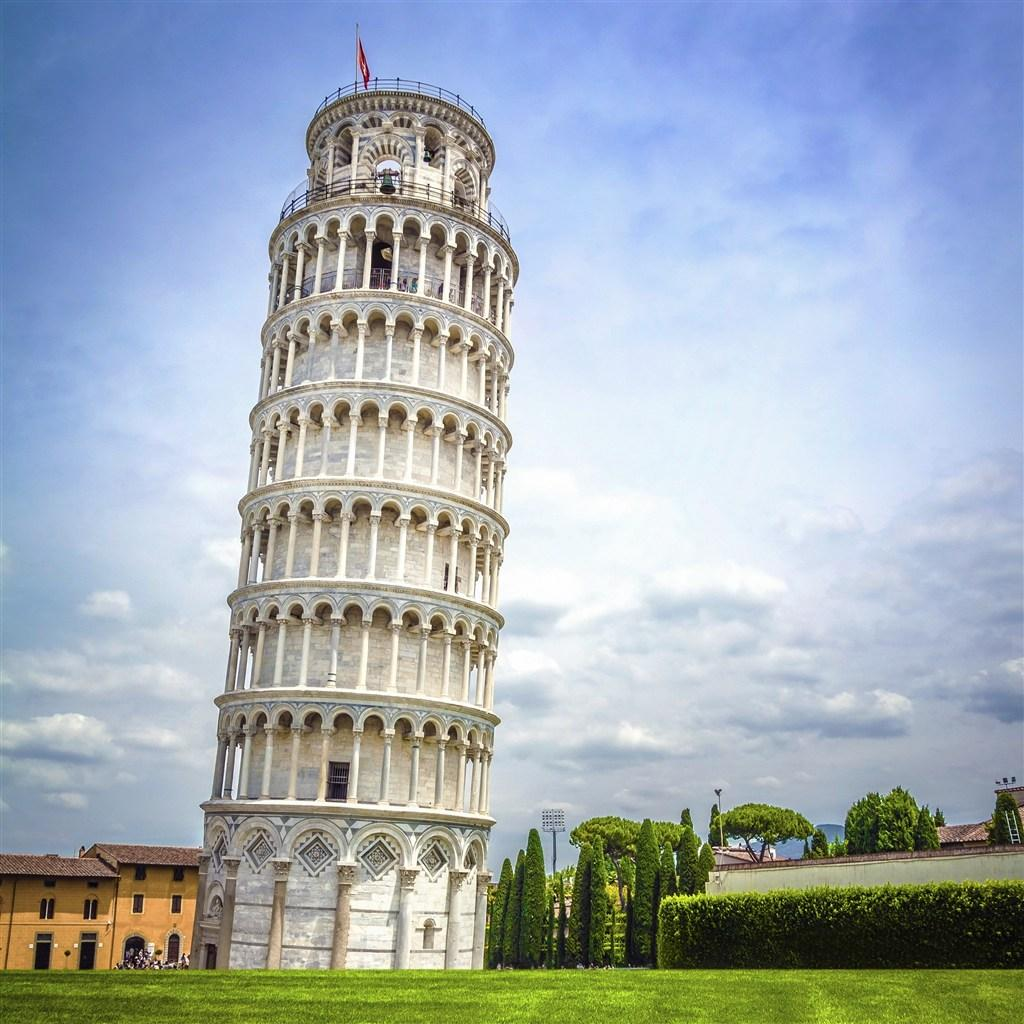
\includegraphics[width=\textwidth]{pisa.jpg}
    \caption{Original}
\end{subfigure}
\begin{subfigure}[b]{0.30\linewidth}
    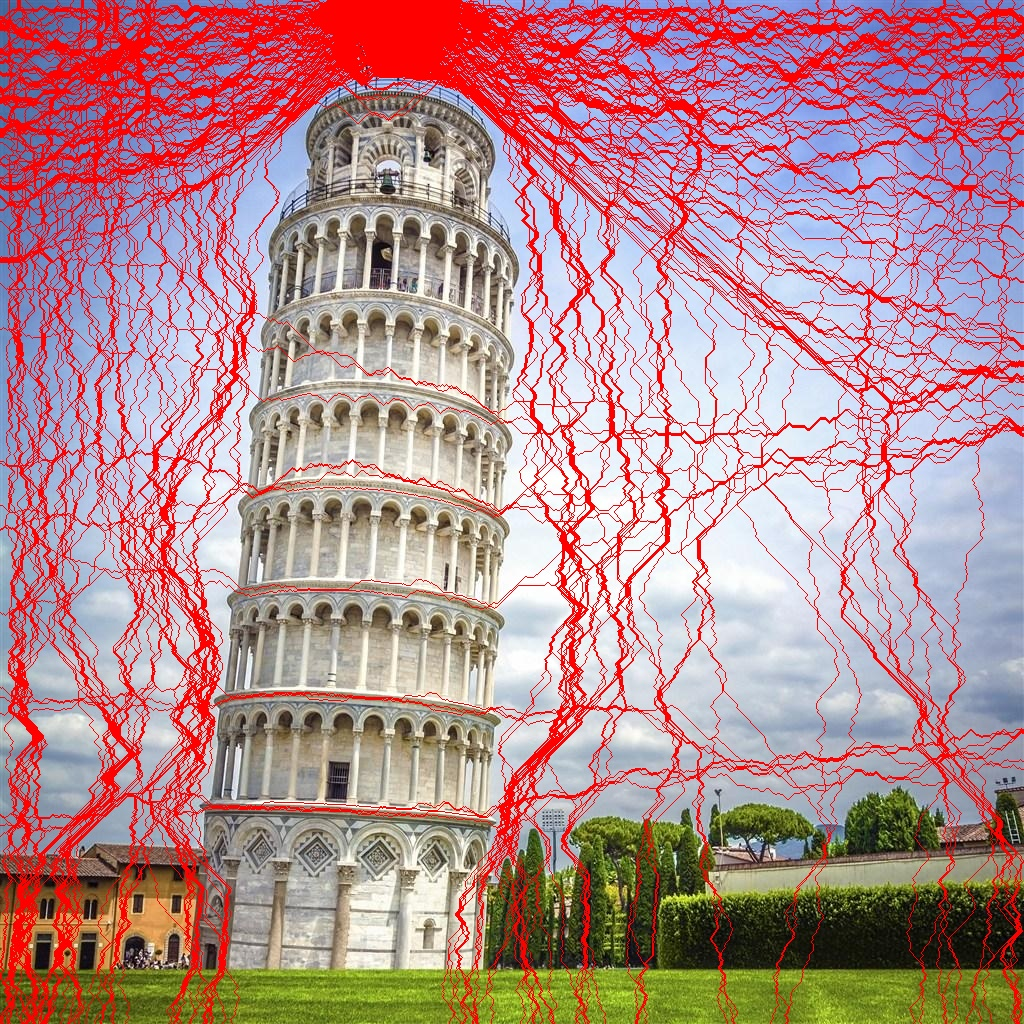
\includegraphics[width=\textwidth]{pisa_seam_carving_width_first_records.jpg}
    \caption{Width-first}
\end{subfigure}
\begin{subfigure}[b]{0.30\linewidth}
    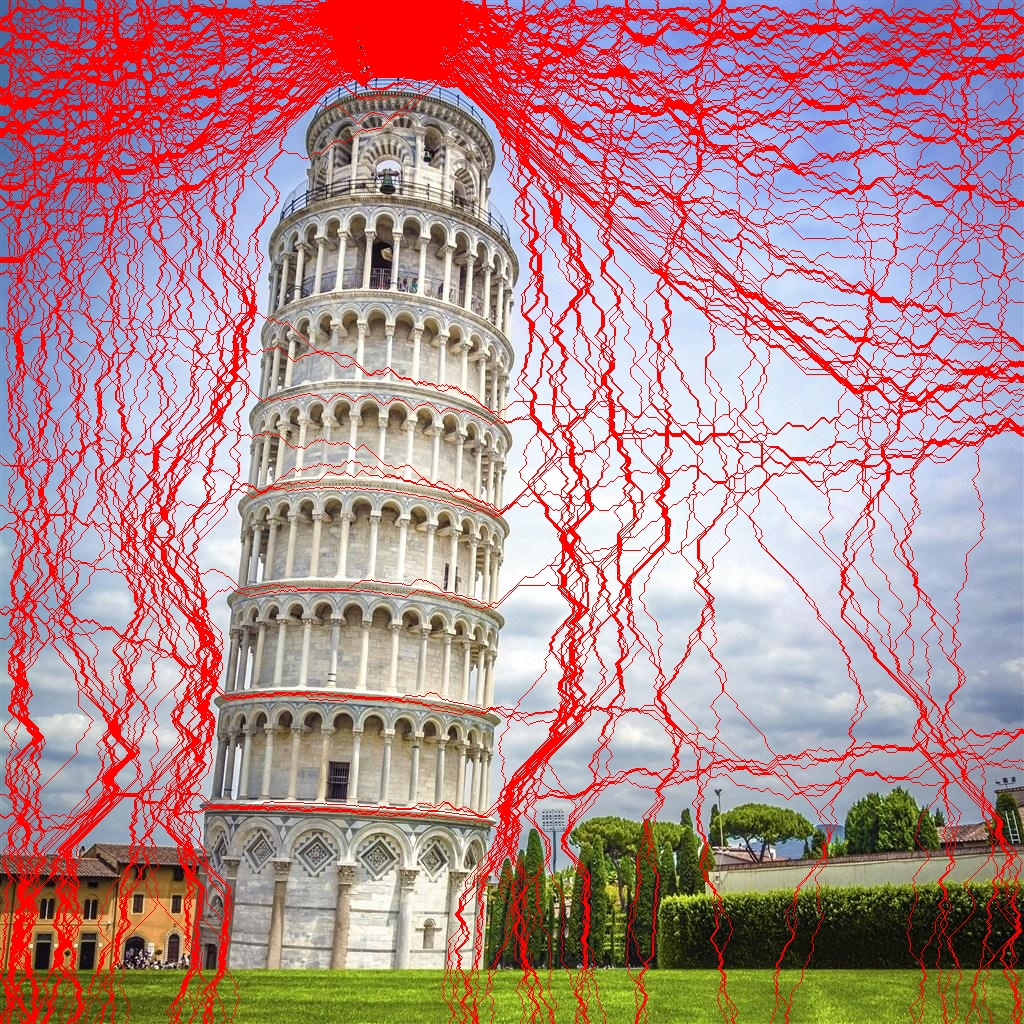
\includegraphics[width=\textwidth]{pisa_seam_carving_height_first_records.jpg}
    \caption{Height-first}
\end{subfigure}
\begin{subfigure}[b]{0.30\linewidth}
    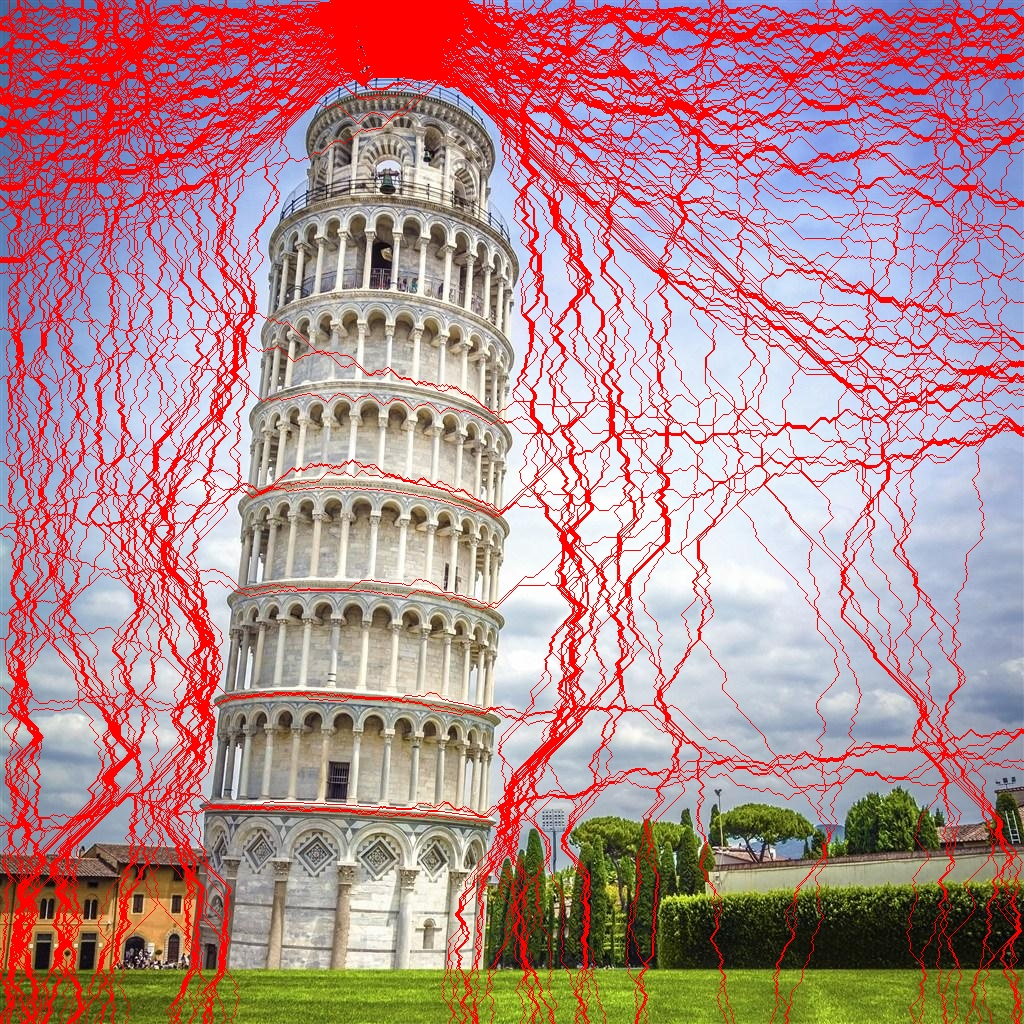
\includegraphics[width=\textwidth]{pisa_seam_carving_optimal_order_records.jpg}
    \caption{Optimal-order}
\end{subfigure}
\begin{subfigure}[b]{0.30\linewidth}
    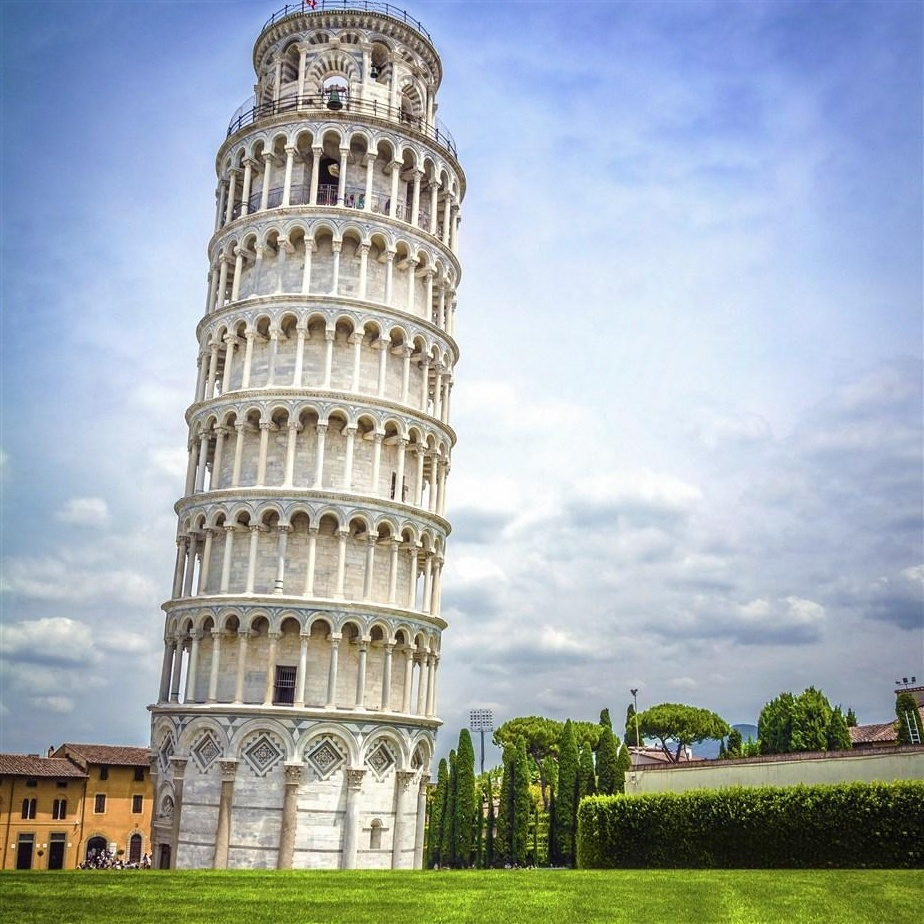
\includegraphics[width=\textwidth]{pisa_seam_carving_width_first.jpg}
    \caption{Width-first}
\end{subfigure}
\begin{subfigure}[b]{0.30\linewidth}
    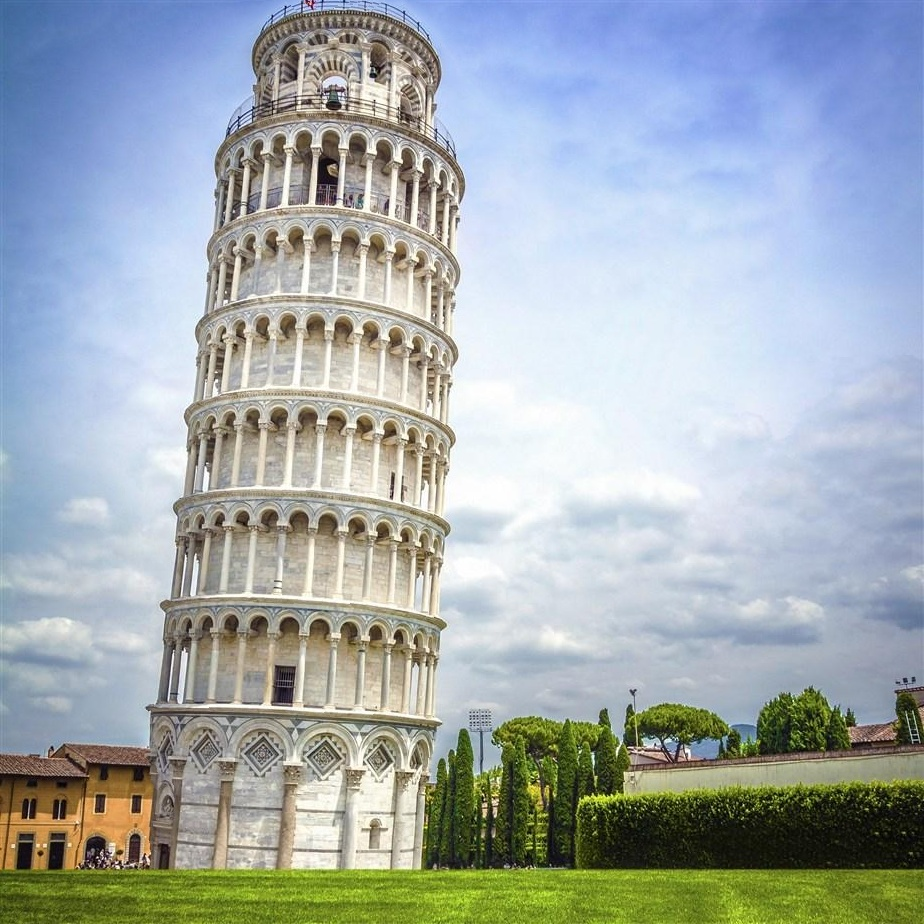
\includegraphics[width=\textwidth]{pisa_seam_carving_height_first.jpg}
    \caption{Height-first}
\end{subfigure}
\begin{subfigure}[b]{0.30\linewidth}
    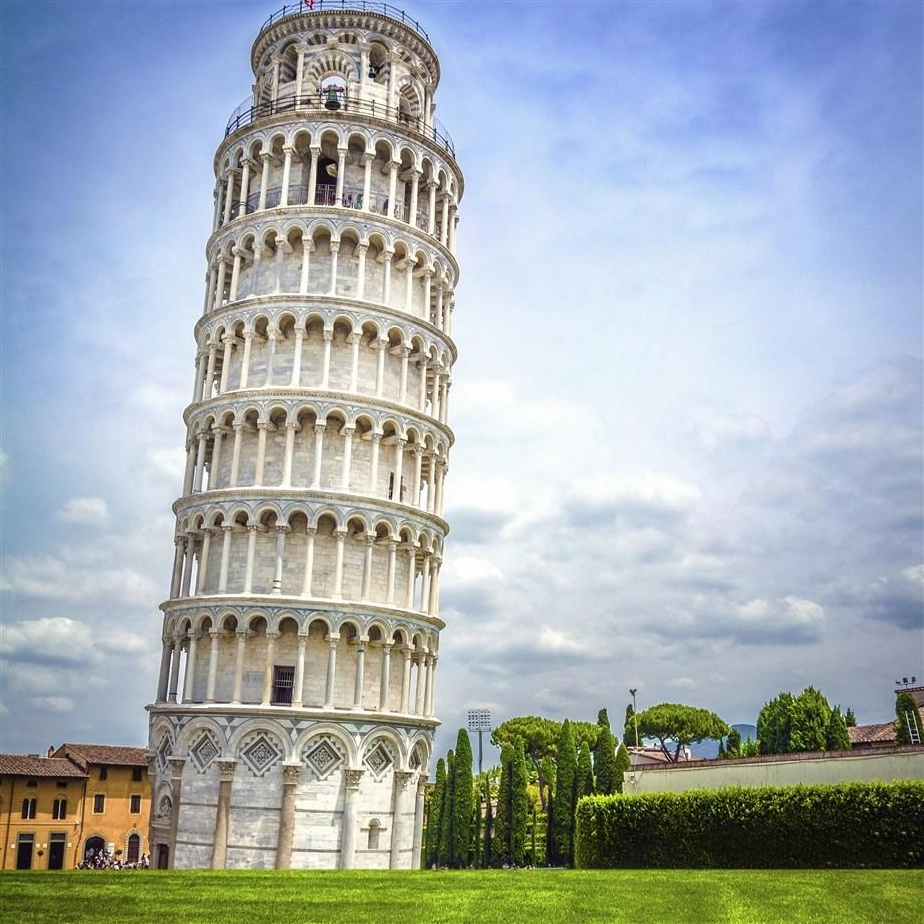
\includegraphics[width=\textwidth]{pisa_seam_carving_optimal_order.jpg}
    \caption{Optimal-order}
\end{subfigure}
\end{center}
\caption{Comparison among width-first, height-first and optimal-order seam carving}
\label{fig:pisa_optimal_order}
\end{figure}
\subsection{Forward Energy}
The paper\cite{rubinstein2008improved} provides a new criterion for choosing the optimal seam.
Energy will be inserted into the graph after the removal of seams, since some of the pixels that are not adjacent in the previous image become adjacent after the removal.
In order to consider the inserted energy after the removal, we regard energy inserted to be the new inserted edges, which has three cases\ref{fig:inserted_edges}.
\begin{figure}[htb]
\begin{center}
\begin{subfigure}[b]{0.30\linewidth}
    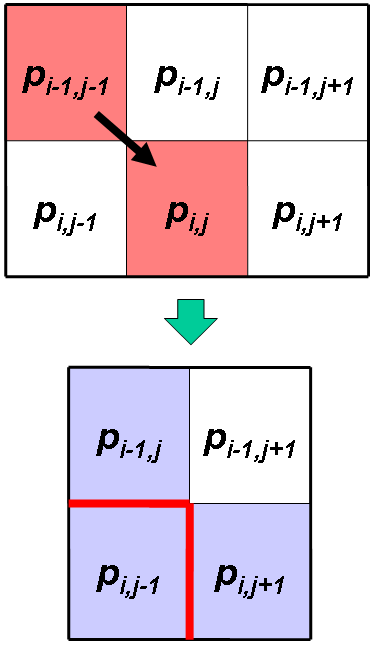
\includegraphics[width=\textwidth]{edge0.png}
    \caption{L-edge}
\end{subfigure}
\begin{subfigure}[b]{0.30\linewidth}
    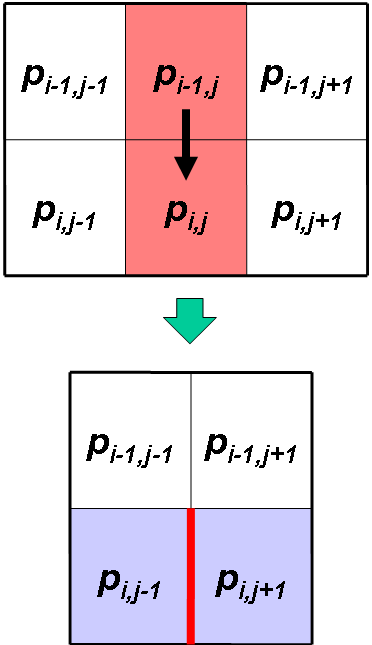
\includegraphics[width=\textwidth]{edge1.png}
    \caption{V-edge}
\end{subfigure}
\begin{subfigure}[b]{0.30\linewidth}
    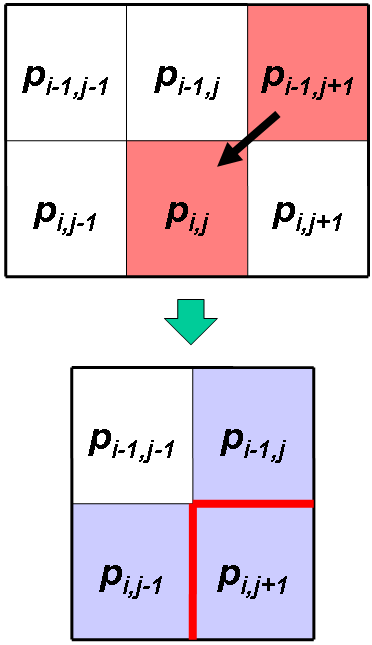
\includegraphics[width=\textwidth]{edge2.png}
    \caption{R-edge}
\end{subfigure}
\end{center}
\caption{Three types of inserted edges}
\label{fig:inserted_edges}
\end{figure}
For the three types of inserted edges, we define three kinds of cost function as follows.
\begin{equation}
    \begin{aligned}
        C_L(i,j)=&|I(i,j+1)-I(i,j-1)|+|I(i-1,j)-I(i,j-1)|\\
        C_V(i,j)=&|I(i,j+1)-I(i,j-1)|\\
        C_R(i,j)=&|I(i,j+1)-I(i,j-1)|+|I(i-1,j)-I(i,j+1)|
        \label{eq:inserted_energy}
    \end{aligned}
\end{equation}
\begin{equation}
\end{equation}
The cost\ref{eq:inserted_energy} is used to replace another way to calculate $e_1$, so the $M$ can be written as
\begin{equation}
    M(i,j)=\min
    \begin{cases}
        M(i-1,j-1)+C_L(i,j)\\
        M(i-1,j)+C_V(i,j)\\
        M(i-1,j+1)+C_R(i,j)
    \end{cases}
    \label{eq:forward_transition_function}
\end{equation}
The comparison between seam carving using forward energy and backward energy is shown in figures.
\begin{figure}[htb]
\begin{center}
\begin{subfigure}[b]{0.70\linewidth}
    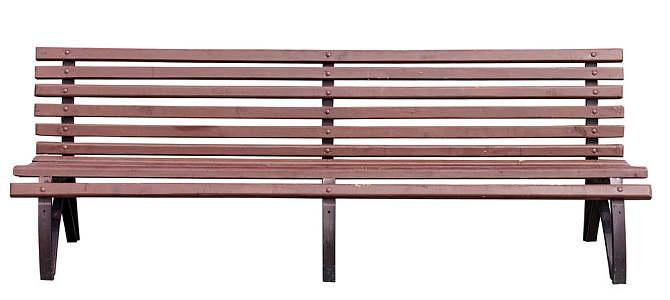
\includegraphics[width=\textwidth]{bench.jpg}
    \caption{Original}
\end{subfigure}
\begin{subfigure}[b]{0.40\linewidth}
    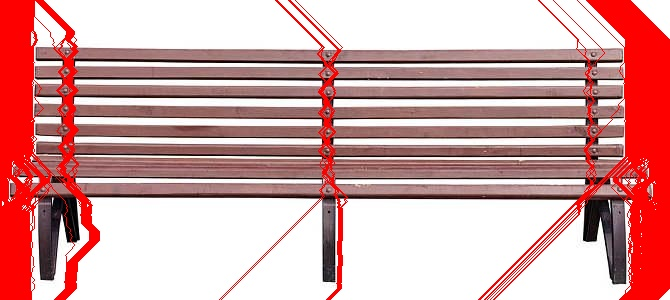
\includegraphics[width=\textwidth]{bench_seam_carving_backward_records.jpg}
    \caption{Backward records}
\end{subfigure}
\begin{subfigure}[b]{0.40\linewidth}
    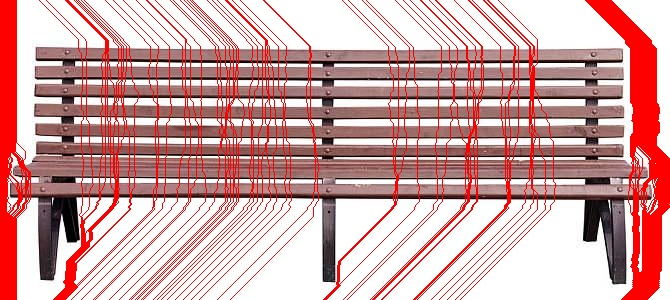
\includegraphics[width=\textwidth]{bench_seam_carving_forward_records.jpg}
    \caption{Forward records}
\end{subfigure}
\begin{subfigure}[b]{0.40\linewidth}
    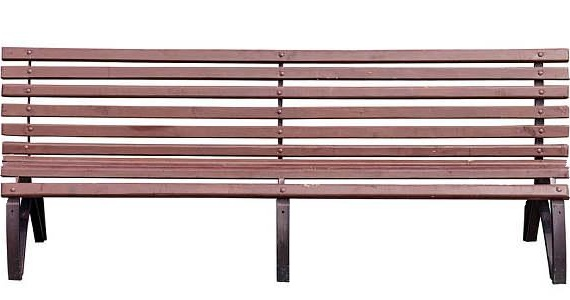
\includegraphics[width=\textwidth]{bench_seam_carving_backward.jpg}
    \caption{Backward results}
\end{subfigure}
\begin{subfigure}[b]{0.40\linewidth}
    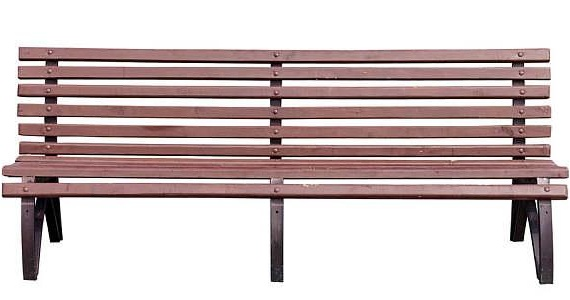
\includegraphics[width=\textwidth]{bench_seam_carving_forward.jpg}
    \caption{Forward results}
\end{subfigure}
\end{center}
\caption{Comparison between backward energy and forward energy}
\label{fig:bench_backward}
\end{figure}

\section{Applications}
The papper\cite{avidan2007seam} gives several interesting applications of seam carving.
Due to the limitation of the this article's length, I select some of the applications that most intrigue me to introduce.
\subsection{Image enlarging}
Image enlarging can be done by the inverse process of image shrinking.
After finding the optimal seam, we duplicate it and average the 2 seams with their neighbors.
However, since the energy of the optimal seam found last time may change very slightly, the optimal seam last time may also be the optimal seam this time.
This may cause constantly duplicating the same seam.
To solve this problem, we can find all the seams that need to be duplicated once and for all, and then duplicate them.
For example, if we want to enlarge the image by $k$, we need to find best $k$ seams and duplicate them.
The comparison of image enlarging between scaling and seam carving is shown in figures\ref{fig:stonehenge_enlarge}.
\begin{figure}[htb]
\begin{center}
\begin{subfigure}[b]{0.70\linewidth}
    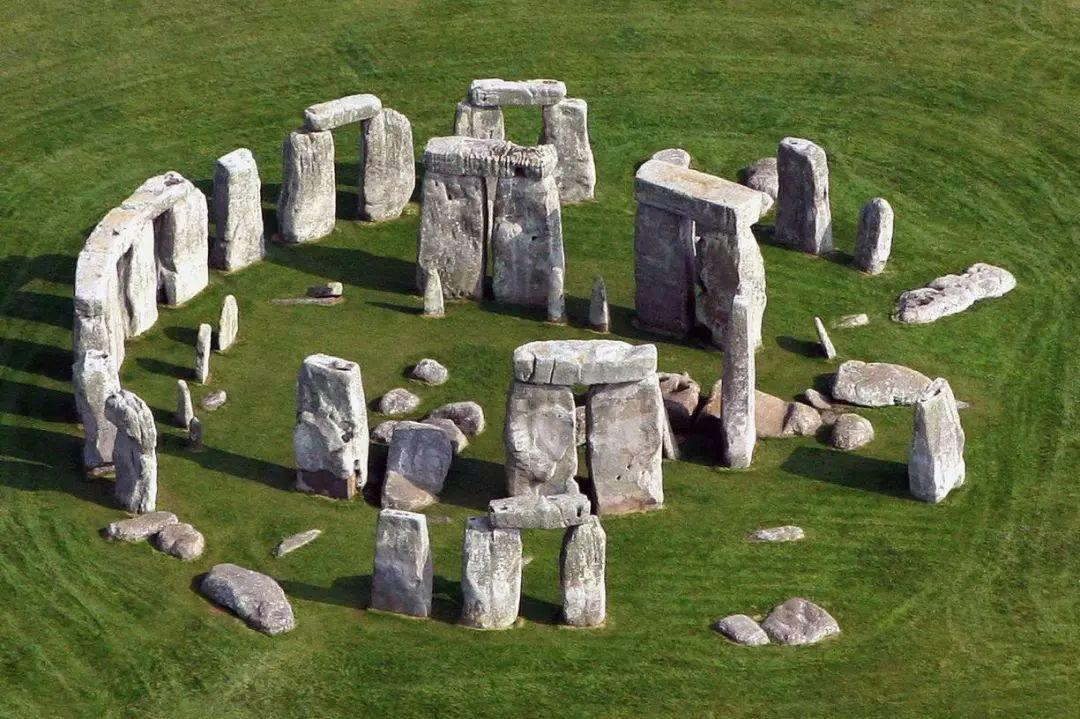
\includegraphics[width=\textwidth]{stonehenge.jpg}
    \caption{Original}
\end{subfigure}
\begin{subfigure}[b]{0.40\linewidth}
    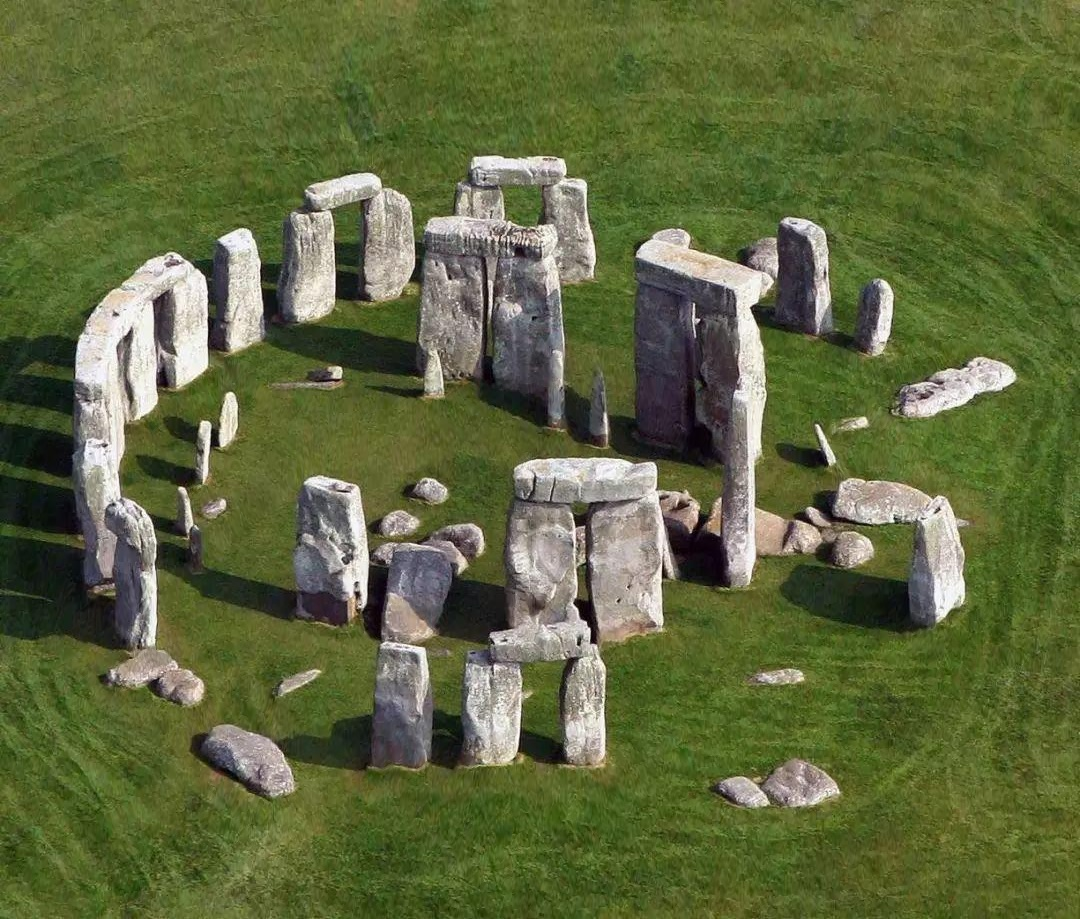
\includegraphics[width=\textwidth]{stonehenge_enlarge.jpg}
    \caption{Scaling}
\end{subfigure}
\begin{subfigure}[b]{0.40\linewidth}
    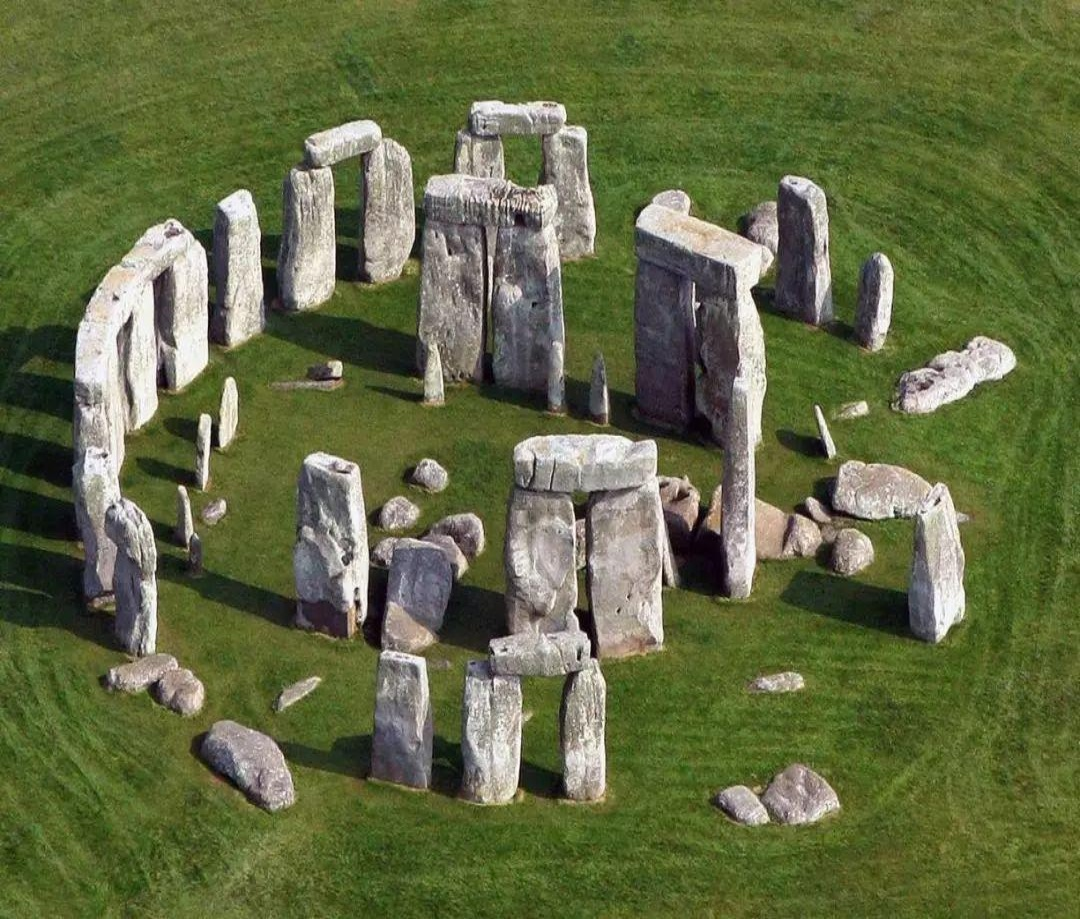
\includegraphics[width=\textwidth]{stonehenge_scale.jpg}
    \caption{Seam carving}
\end{subfigure}
\end{center}
\caption{Comparison of enlarging between scaling and seam carving}
\label{fig:stonehenge_enlarge}
\end{figure}
\subsection{Object removal}
This is similar to energy with masks.
Here we manually decrease energy of pixels on the object that we want to remove.
And we won't stop removing seams until all the pixels on the mask are removed.

The figures\ref{fig:liberty_removal} shows that how seam carving vanishes the statue of liberty.
\begin{figure}[htb]
\begin{center}
\begin{subfigure}[b]{0.40\linewidth}
    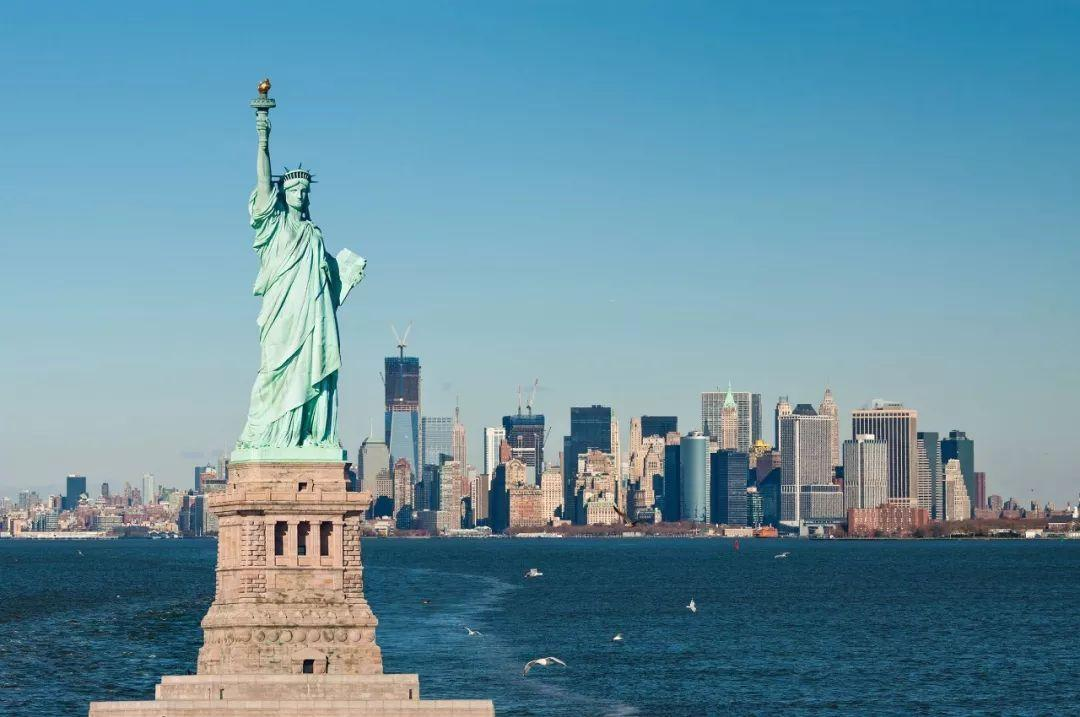
\includegraphics[width=\textwidth]{liberty.jpg}
    \caption{Original}
\end{subfigure}
\begin{subfigure}[b]{0.40\linewidth}
    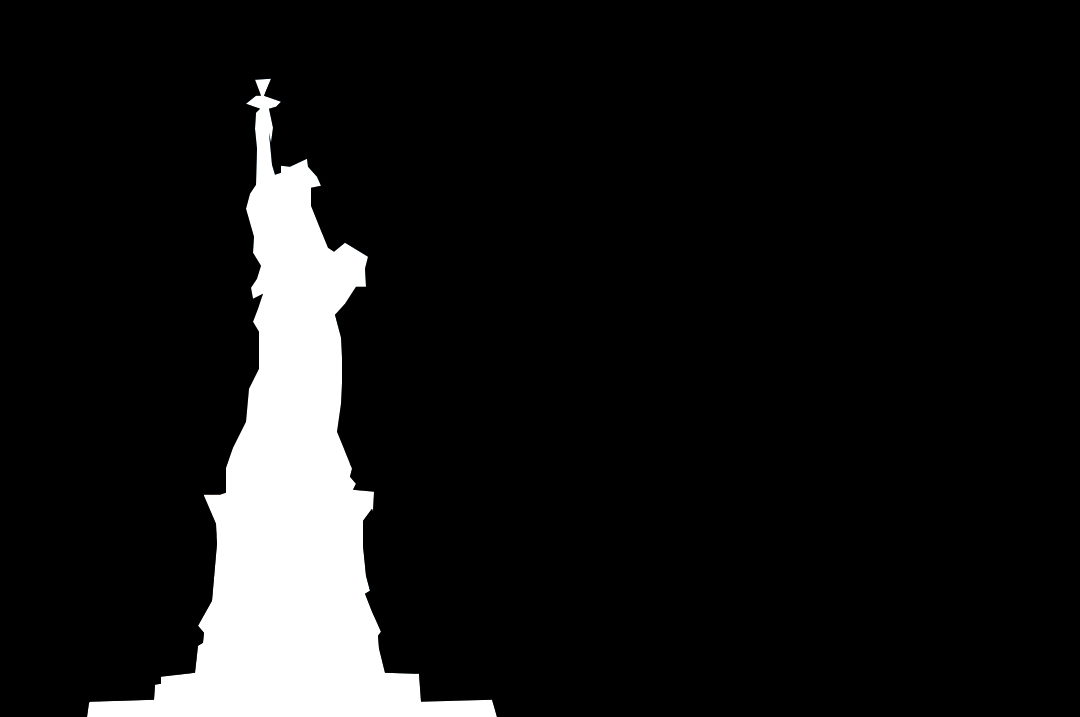
\includegraphics[width=\textwidth]{liberty_mask.jpg}
    \caption{Mask}
\end{subfigure}
\begin{subfigure}[b]{0.70\linewidth}
    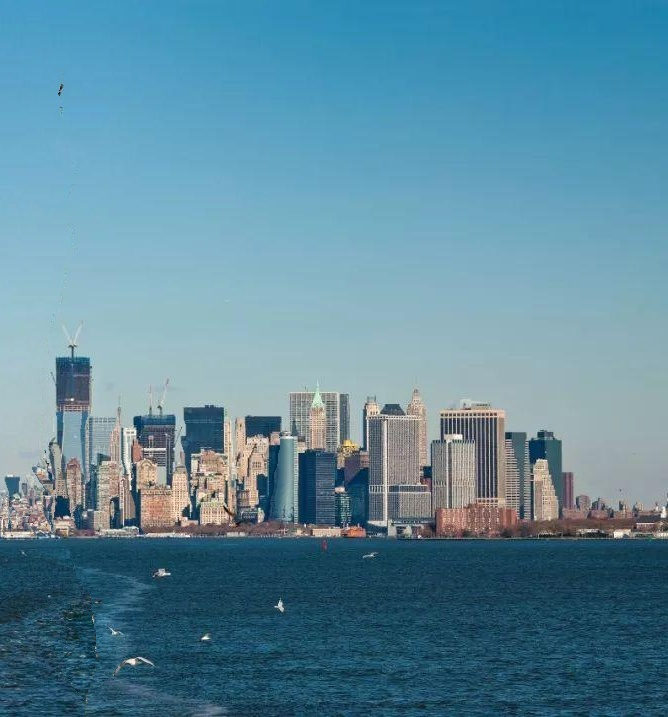
\includegraphics[width=\textwidth]{liberty_removal.jpg}
    \caption{Object removal}
\end{subfigure}
\end{center}
\caption{Comparison of enlarging between scaling and seam carving}
\label{fig:liberty_removal}
\end{figure}
\section{Conclusions}
Thanks to this homework, I have a deeper understanding of the seam carving, and I realized most of the ideas shown in this article.
However, there are still some of the thoughts that I havn't realize, i.e. the parallelization of the seam carving, image enlarging with records and conbine $eHoG$ with forward energy.
Some of them may be realized at the end of the semester.
{\small
\bibliographystyle{ieee_fullname}
\bibliography{egbib}
}

\end{document}
